%% V0.2
%% by Luis Felipe Wolf Batista, luisfelipewb@gmail.com
%% This is a template for Udacity projects using IEEEtran.cls


\documentclass[10pt,journal,compsoc]{IEEEtran}

\usepackage[pdftex]{graphicx}    
\graphicspath{{img/}}
\usepackage{subfig}
\usepackage{cite}
\hyphenation{op-tical net-works semi-conduc-tor}

%%Packages for code snippet
\usepackage{listings}
\usepackage{xcolor}
\lstset { %
    language=C++,
    backgroundcolor=\color{black!5}, % set backgroundcolor
    basicstyle=\footnotesize,% basic font setting
}

\begin{document}

\title{Deep RL Arm Manipulation}

\author{Luis F. W. Batista}

\markboth{Deep RL Arm Manipulation Project, Robotic Nanodegree, Udacity}%
{}
\IEEEtitleabstractindextext{%

\begin{abstract}
Deep Reinforcement Learning combines Reinforcement Learning with Deep Neural Networks to achieve human-level control in several applications. This report explains the parameters used by a DQN agent to teach a robotic arm with three degrees of freedom how to reach a target object. During evaluation success rates above 80\% are achieved.

\end{abstract}

% Note that keywords are not normally used for peerreview papers.
\begin{IEEEkeywords}
Robot, IEEEtran, Udacity, \LaTeX, Deep Learning, DQN, Reinforcement Learning.
\end{IEEEkeywords}}

\maketitle
\IEEEdisplaynontitleabstractindextext
\IEEEpeerreviewmaketitle
\section{Introduction}
\label{sec:introduction}

\IEEEPARstart{D}{eep Reinforcement Learning} is a paradigm shift for Robotics. In summary, the idea is to define a goal for the robot, provide raw sensor input and let it find out the best way to achieve the goal by trial and error. The main difference in this paradigm is that is not necessary to explicitly define the perception, internal state, planning, control, and even sensor measurement uncertainty. All those traditional steps necessary to take proper action are learned by a neural network. 

\section{Background / Formulation}
This project is part of the Robotics Software Engineer Nanodegree Program - Term 2 from Udacity. The goal is to create a DQN agent and define reward functions to teach a robotic arm to carry out two primary objectives: 

\begin{enumerate}
  \item Have any part of the robot arm touch the target object with at least 90\% accuracy.
  \item Have only the gripper base of the robot arm touch the target object with at least 80\% accuracy.
\end{enumerate}

In this report, the first objective is referred to as "Arm Collision", where the second is "Gripper Collision"
Both goals are accomplished in a simulated environment through the development of a C++ plugin for Gazebo.





\section{Reward Functions}


The reward function definition is very important to guarantee the convergence of the reinforcement learning algorithm. In this project, the following types were defined.

\begin{itemize}
  \item REWARD\_WIN: Final reward when the target is reached.
  \item REWARD\_LOSS: Negative reward when the robot touches the ground.
  \item REWARD\_TIMEOUT: Negative reward when the maximum iteration is reached.
  \item REWARD\_CLOSER: Positive reward when the gripper moves closer to the target
  \item REWARD\_FARTHER: Negative reward when the gripper moves away from the target
\end{itemize}

The value for each reward was selected based on experimentation. The description can be found in the following subsections. 

\subsection{Arm Collision}

The REWARD\_WIN was issued when any part of the robot touched the target.
\begin{lstlisting}
if (collisionCheckArm)
{
	rewardHistory = REWARD_WIN;
	newReward  = true;
	endEpisode = true;

	return;
}
\end{lstlisting}

The rewards based on the distance of the gripper and target used a smoothed average of the distance variation. It can be seen on the following code snippet.
\begin{lstlisting}
// compute the smoothed moving average
avgGoalDelta  = (avgGoalDelta * 0.05) + 
                (distDelta * 0.95);
if (avgGoalDelta > 0)
	rewardHistory = REWARD_CLOSER;
else
	rewardHistory = REWARD_FARTHER;				
\end{lstlisting}

The values for the reward functions were defined as follows. 
\begin{lstlisting}
#define REWARD_WIN  100.0f
#define REWARD_LOSS -50.0f
#define REWARD_TIMEOUT -10.0f
#define REWARD_CLOSER 1.0f
#define REWARD_FARTHER -2.0f
\end{lstlisting}

High values were selected for the final rewards as an incentive for the agent to learn how to reach the goal. It prevents the learning process to prioritize intermediate rewards.

The intermediary rewards guide the robot by providing incentives when it is moving towards the correct direction. The penalty when moving farther is stronger than the reward to move closer. The intention is to prevent the robot to oscillate in the same place. A penalty based on elapsed time could provide similar results.

For the first goal, the type of joint control was based on the position of the arm. 
\begin{lstlisting}
#define VELOCITY_CONTROL false	
\end{lstlisting}

Additionally, the delta was decreased by one third to guarantee a smooth arm movement.
\begin{lstlisting}
actionJointDelta = 0.05f;
\end{lstlisting}


\subsection{Gripper Collision}

A similar approach was used to select the reward values when the accepted collision point was restricted to the gripper. The value selected for the parameters were:
\begin{lstlisting}
#define REWARD_WIN  100.0f
#define REWARD_LOSS -100.0f
#define REWARD_TIMEOUT -50.0f
#define REWARD_CLOSER 10.0f
#define REWARD_FARTHER -20.0f
\end{lstlisting}

The first difference was that a penalty was issued when the robotic arm touched the target with a link other than the gripper. It was necessary to avoid situations when the middle of the arm was touching the target and the episode did not finish. 
\begin{lstlisting}
if (collisionCheckGripper)
{
	rewardHistory = REWARD_WIN;
	
	newReward  = true;
	endEpisode = true;

	return;
}
if (collisionCheckArm)
{
	rewardHistory = REWARD_LOSS;
	
	newReward  = true;
	endEpisode = true;

	return;
}
\end{lstlisting}


The second difference was that the intermediate rewards were based directly on the distance variation, instead of the smoothed average. This was based on the assumption that the arm can always move towards the final goal. 
\begin{lstlisting}
if (distDelta > 0.0)
	rewardHistory = REWARD_CLOSER;
	
else
	rewardHistory = REWARD_FARTHER;
\end{lstlisting}

Finally, the type of joint control was based on the velocity of the joints. To guarantee a smooth arm movement, the velocity delta and maximum speed were decreased.
\begin{lstlisting}
#define VELOCITY_CONTROL true	
#define VELOCITY_MIN -0.05f
#define VELOCITY_MAX  0.05f
\end{lstlisting}

Similarly to the previous goal, the velocity increment was also reduced as follows. 
\begin{lstlisting}
actionVelDelta   = 0.05f;
\end{lstlisting}


\section{Hyperparameters}

To achieve higher accuracy the hyper-parameters for the Neural Network were defined as follows:
\begin{lstlisting}
#define INPUT_WIDTH   64
#define INPUT_HEIGHT  64
#define OPTIMIZER "RMSprop"
#define LEARNING_RATE 0.1f // 0.001 for second goal
#define REPLAY_MEMORY 20000
#define BATCH_SIZE 32	
#define USE_LSTM true
#define LSTM_SIZE 256
\end{lstlisting}

The only difference between each goal was the LEARNING\_RATE. The reason for decreasing the learning rate from 0.1 to 0.001 was to prevent overfitting during the learning process. 

The INPUT\_WIDTH and the INPUT\_HEIGHT parameters were defined according to the image resolution used in the simulation.

"RMSprop" was selected as the OPTIMIZER since it provided better results than "Adam". 

The use of Long Short Term Memory was enabled to take into consideration multiple past frames from the camera sensor instead of a single frame.

The remaining parameters were defined empirically to increase accuracy.



\section{Results}

\subsection{Arm Collision}

Due to the simplicity of the task, the robot learned fairly quickly that it was sufficient to only rotate the joint between the base and the first link to achieve the goal. 

As a result, the minimum of 90\% accuracy could be achieved after 10 episodes. The Figure \ref{fig:arm_collision} shows final accuracy above 99\% after 100 episodes.

\begin{figure}[thpb]
      \centering
      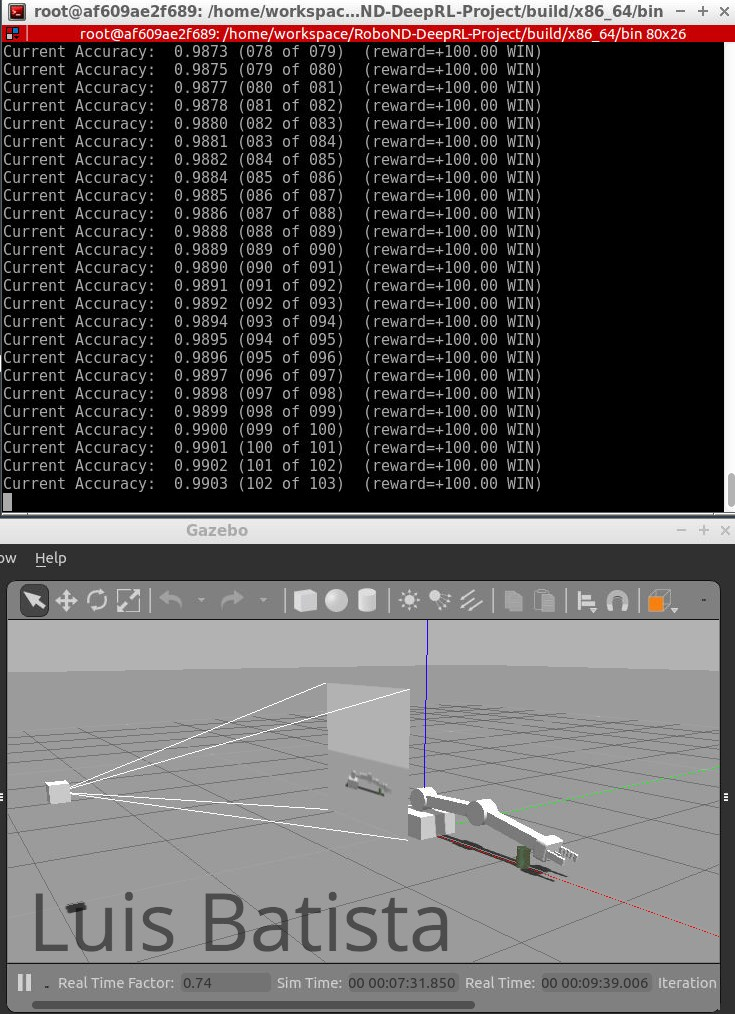
\includegraphics[width=\linewidth]{arm_collision.png}
      \caption{Arm Collision Accuracy}
      \label{fig:arm_collision}
\end{figure}


\subsection{Gripper Collision}
It was more complex to train the robot to reach the target touching only the gripper.

The lower learning rate resulted in longer training time to achieve the minimum requirements. 

The Figure \ref{fig:gripper_collision} shows the accuracy surpassing the 80\% requirement after 380 episodes.

\begin{figure}[thpb]
      \centering
      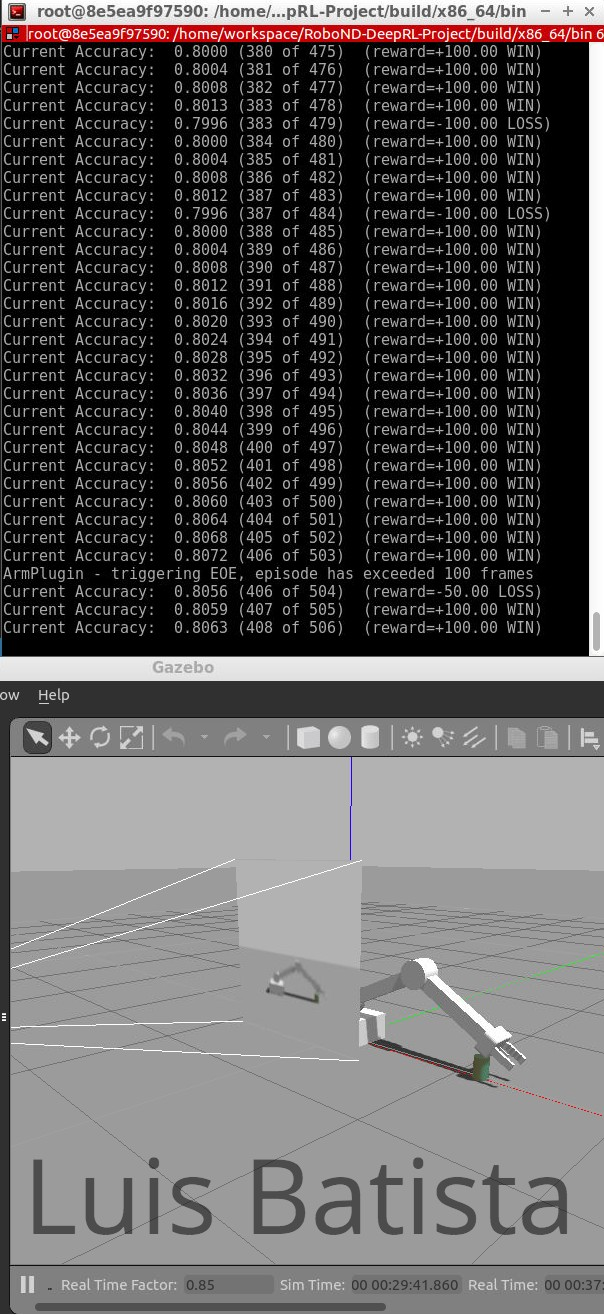
\includegraphics[width=\linewidth]{gripper_collision.png}
      \caption{Gripper Collision Accuracy}
      \label{fig:gripper_collision}
\end{figure}


\section{Future work}

The required accuracy was achieved, but it is still possible to optimize the results especially for the Gripper Collision goal.  Such optimization could be done by further adjusting the parameters including learning rate and LSTM values or also implementing more robust reward functions.

To make the problem more realistic scenarios, it is possible to train the agent when the target is in random locations and allow the robot to with additional degrees of freedom.

\end{document}

